\section{Introduction}
\label{sec:intro}

In many proposals to attain BGP~\cite{bgp}
security~\cite{s-bgp1,s-bgp2,sobgp,psbgp,spv}, such as
SIDR~\cite{sidr-arch}, an address assignment authority signs resource
certificates for address spaces and autonomous system
numbers.

Ideally, a single authority would sign every resource certificate. A
single signer could easily ensure that the signed certificates did not
conflict; for example, no two certificates would assign the same
address space to different parties. However, political considerations
seem to preclude this solution in the case of
address space and autonomous system number resource certificates.

An alternate solution involves each of the five regional internet
registries (RIRs) acting as independent certificate authorities. Each
RIR would agree to sign certificates only for their own address
space. Unfortunately, this approach is far more complex in practice:
preventing accidental address space allocation overlap or accidental
removal of address allocations across multiple RIRs is hindered in
such a stove-piped solution.  In addition, at least five public keys
(one for each RIR) must be distributed to and updated by all
verifiers. While verifiers must obtain and trust some public key in
order to verify the validity of certificates, increasing the number of
necessary trust anchors greatly increases the complexity of the system
for verifiers and can reduce security.

In order to obtain many of the benefits of a single signing authority
while allowing the RIRs to retain their autonomy, in this paper we
outline procedures to allow multiple players to operate a single {\it
virtual} signing authority as a {\it root collective}. This virtual
signing authority would have a single public key, making it appear as
a single signing authority to verifiers, but signing would be
cooperatively performed by some subset of the players. The RIRs appear
to be operationally suitable to form the root collective. We
illustrate the process of creating a signature in
Figure~\ref{fig:sign-combine}.

The virtual signing authority must be:
\begin{itemize}
\item {\bf Secure.} If the private (signing) key is leaked or
otherwise obtained by an adversary, that adversary can sign erroneous
data. We refer to such keys as {\it compromised}. The virtual signing
authority must be at least as secure as a single signing authority,
including the ability to utilize existing hardware security modules
for protection of the secret key. In fact, our scheme for a virtual
signing authority can be considered more secure, as more than one
secret key must be leaked in order to break the scheme.

\item {\bf Invisible.} No verifier should need to know the
administrative arrangements of the certificate signing
system. Signatures on certificates are verified from a single trust
anchor just as if there was a single signing authority instead of a
virtual signing authority.

\item {\bf Efficient.} Signing certificates should not be a heavy
burden on the members of the root collective. In particular, the
amount of interactive communication during signing should be minimal:
one player distributes data to be signed and the other players return
{\it signature shares}, which can be combined into a complete signature,
valid under the virtual signer's public key. In addition, our scheme
for a virtual signing authority can actually increase availability
over a single signer, because not all players in the root collective
must be available to produce a signature.
\end{itemize}

\ignore{

\begin{figure}
\begin{center}
\fbox{
\begin{minipage}{5in}
\centerline{
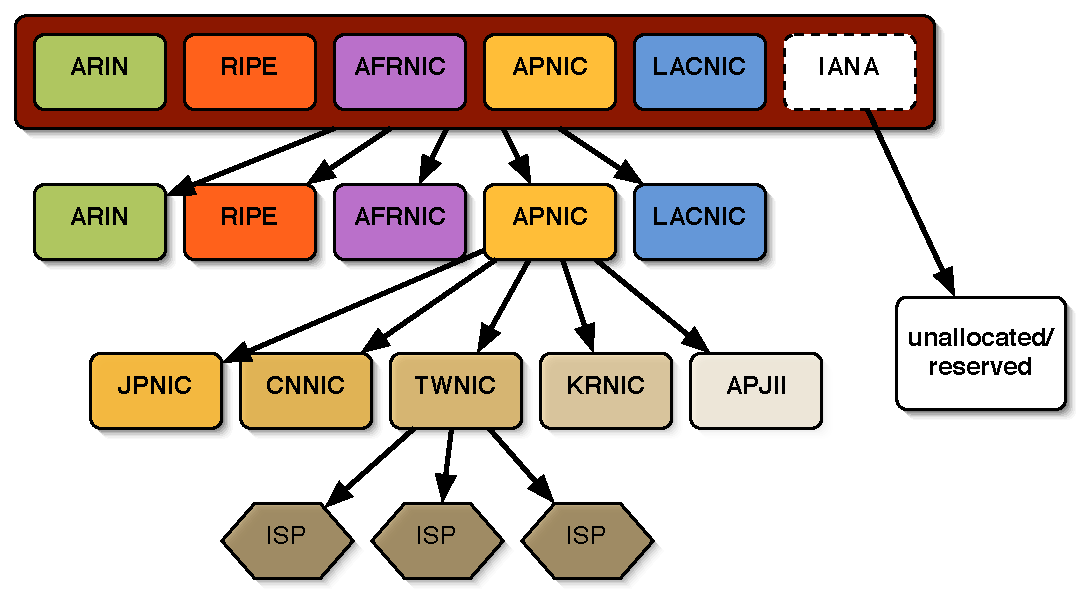
\includegraphics[width=5in]{figures/pki-hierarchy} 
}
\end{minipage}

}% FBOX
\end{center}
\caption{\small The address PKI root should be managed by the five RIRs in collaboration with IANA. The root of the hierarchy signs certificates allowing each RIR to securely manage its allocated address space. Each RIR, in turn, signs certificates for the address allocations of  ISPs and/or country registries, who may delegate sections of the address space in turn.}
\label{fig:hierarchy}
\end{figure}

}

\begin{figure}
\begin{center}
\fbox{
\begin{minipage}{5in}
\centerline{
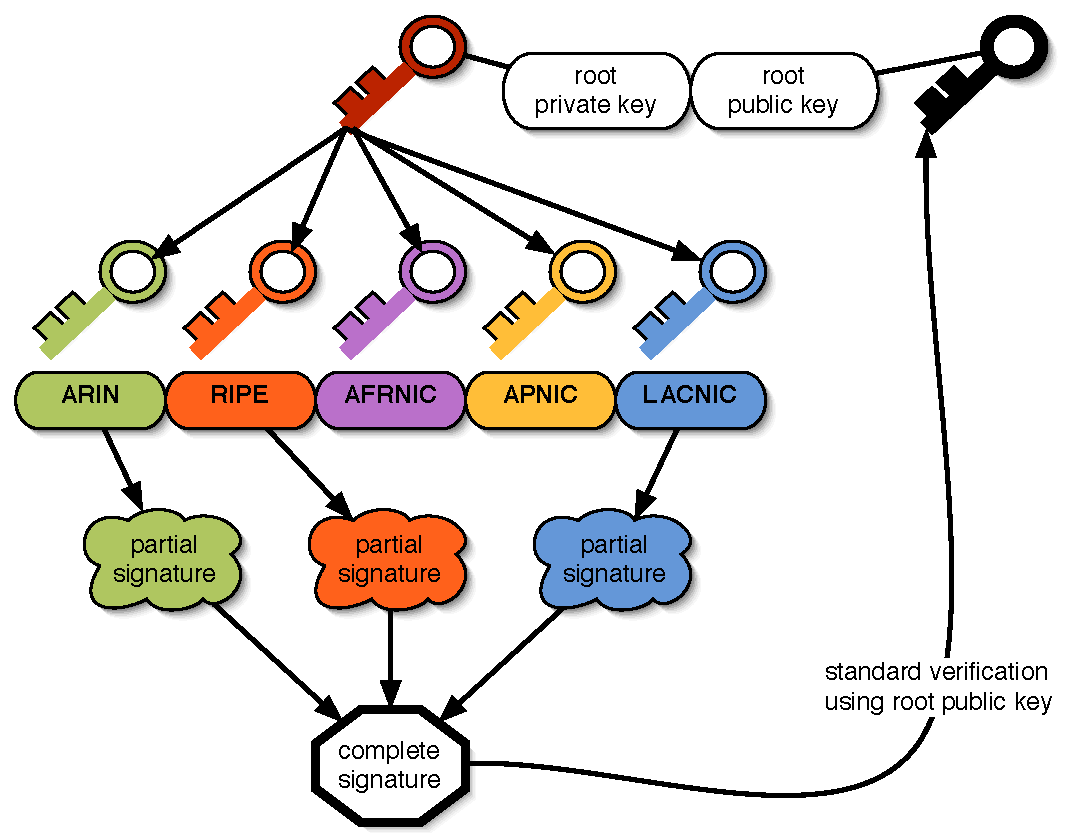
\includegraphics[width=5in]{figures/sign-combine} 
}
\end{minipage}

}% FBOX
\end{center}
\caption{\small The distributed root of a PKI functions as follows:
(1) a trusted dealer chooses a root public and private (signing) key;
(2) the dealer creates shares of the signing key for each player/RIR;
(3) to create a signature, at least $\nums=3$ players create signature
shares from their key shares and combine them into a complete
signature; (4) the complete signature can be verified with the root
public key, just as if it were created directly from the root private
key.}
\label{fig:sign-combine}
\end{figure}
